\subsection{Roviny v prostoru}
\label{subsec:Planes_in_space}

Rovina je nekonečný rovinný útvar, který se rozprostírá ve dvou navzájem
nezávislých směrech. Zatímco k určení přímky potřebujeme jeden bod a jeden
směr, k určení roviny potřebujeme jeden bod a dva různé směry, které
nejsou navzájem rovnoběžné.

Uvažujme bod
\[
    A[x_A;y_A;z_A]
\]
a dva nenulové, navzájem nerovnoběžné vektory
\[
    \vec{u}=(u_x;u_y;u_z),
    \qquad
    \vec{v}=(v_x;v_y;v_z).
\]
Vektory $\vec{u}$ a $\vec{v}$ určují dva směry ležící v rovině. Jejich
lineárními kombinacemi se můžeme z bodu $A$ dostat do libovolného dalšího
bodu této roviny.

\begin{figure}[H]
    \centering
    \begin{tikzpicture}[scale=0.9]

        % Rovina
        \coordinate (P1) at (-1,0,0.5);
        \coordinate (P2) at (3,1,0.5);
        \coordinate (P3) at (4,3,2.5);
        \coordinate (P4) at (0,2,2.5);

        \fill[gray!18] (P1) -- (P2) -- (P3) -- (P4) -- cycle;
        \draw[thin] (P1) -- (P2) -- (P3) -- (P4) -- cycle;

        % Osy - kladná část
        \draw[->] (0,0,0) -- (4.8,0,0) node[right] {$x$};
        \draw[->] (0,0,0) -- (0,4.3,0) node[above] {$y$};
        \draw[->] (0,0,0) -- (0,0,3.8) node[below left] {$z$};

        % Osy - záporná část
        \draw[->, dashed] (0,0,0) -- (-2.2,0,0);
        \draw[->, dashed] (0,0,0) -- (0,-2.2,0);
        \draw[->, dashed] (0,0,0) -- (0,0,-2.6);

        \node[above left] at (0,0,0) {$O$};

        % Bod a směrové vektory roviny
        \coordinate (A) at (1.4,1.3,1.3);
        \coordinate (U) at (3.8,1.9,1.3);
        \coordinate (V) at (2,2.5,2.5);

        \draw[vector] (A) -- (U)
            node[midway, sloped, above] {$\vec{u}$};
        \draw[vector] (A) -- (V)
            node[midway, sloped, above] {$\vec{v}$};

        \fill (A) circle (2pt) node[below left] {$A$};
        \node at (3.65,2.75,2.35) {$\alpha$};

    \end{tikzpicture}
    \caption{Rovina $\alpha$ určená bodem $A$ a dvěma navzájem
    nerovnoběžnými směrovými vektory $\vec{u}$ a $\vec{v}$.}
    \label{fig:Plane_point_two_vectors}
\end{figure}

Podobně jako přímku lze i rovinu určit několika různými způsoby. Rovinu
jednoznačně určují například:

\begin{itemize}
    \item jeden bod a dva navzájem nerovnoběžné směrové vektory;
    \item tři body, které neleží na jedné přímce;
    \item přímka a bod, který na této přímce neleží;
    \item dvě různoběžné přímky;
    \item dvě různé rovnoběžné přímky.
\end{itemize}

Podmínky uvedené v jednotlivých případech jsou důležité. Tři body ležící
na jedné přímce například rovinu jednoznačně neurčují, protože danou
přímkou prochází nekonečně mnoho rovin. Stejně tak dva rovnoběžné směrové
vektory určují pouze jeden směr, a nestačí proto k popsání celé roviny.

Roviny budeme popisovat dvěma základními způsoby:

\begin{itemize}
    \item \textbf{parametrickým vyjádřením}, které využívá jeden bod
    roviny a dva její směrové vektory;
    \item \textbf{obecnou rovnicí roviny}, která využívá normálový vektor
    kolmý k rovině.
\end{itemize}

Nejprve se zaměříme na parametrické vyjádření roviny, které přímo navazuje
na parametrické vyjádření přímky a na lineární kombinace vektorů.


\subsection{Parametrické vyjádření roviny}
\label{subsec:Parametric_plane}

Rovina je určena jedním bodem a dvěma navzájem nezávislými směry.
Z výchozího bodu se tedy můžeme pohybovat současně ve směru dvou
nenulových, navzájem nerovnoběžných vektorů.

Uvažujme bod
\[
    A[x_A;y_A;z_A]
\]
a dva nenulové, navzájem nerovnoběžné vektory
\[
    \vec{u}=(u_x;u_y;u_z),
    \qquad
    \vec{v}=(v_x;v_y;v_z).
\]

Libovolný bod $X[x;y;z]$ roviny získáme z bodu $A$ posunutím o vhodný
násobek vektoru $\vec{u}$ a vhodný násobek vektoru $\vec{v}$:
\[
    X=A+s\vec{u}+t\vec{v},
\]
kde $s,t\in\mathbb{R}$.


\subsubsection{Rovina určená bodem a dvěma směrovými vektory}
\label{subsubsec:Plane_point_two_direction_vectors}

\begin{definition}
    \label{def:Parametric_plane}

    Nechť $A[x_A;y_A;z_A]$ je bod v prostoru a nechť
    \[
        \vec{u}=(u_x;u_y;u_z),
        \qquad
        \vec{v}=(v_x;v_y;v_z)
    \]
    jsou dva nenulové, navzájem nerovnoběžné vektory.

    Rovina $\alpha$ procházející bodem $A$ a mající směrové vektory
    $\vec{u}$ a $\vec{v}$ je množina všech bodů $X$, které lze vyjádřit
    ve tvaru
    \begin{equation}
        X=A+s\vec{u}+t\vec{v},
        \qquad
        s,t\in\mathbb{R}.
        \label{eq:Parametric_plane_vector}
    \end{equation}

    Po rozepsání do souřadnic získáme parametrické rovnice roviny
    \begin{equation}
        \begin{aligned}
            \alpha: x&=x_A+s u_x+t v_x,\\
            y&=y_A+s u_y+t v_y,\\
            z&=z_A+s u_z+t v_z; \quad s,t\in\mathbb{R}.
        \end{aligned}
        \label{eq:Parametric_plane_coordinates}
    \end{equation}

    Parametry $s$ a $t$ jsou opět známými \textbf{parametry roviny} a vektory
    $\vec{u}$ a $\vec{v}$ jejími \textbf{směrovými vektory}.
\end{definition}

Vektor směřující z bodu $A$ do libovolného bodu $X$ roviny má tvar
\begin{equation}
    \overrightarrow{AX}=s\vec{u}+t\vec{v}.
    \label{eq:Plane_displacement_vector}
\end{equation}

Každý vektor spojující bod $A$ s bodem roviny je tedy lineární kombinací
jejích směrových vektorů.

\begin{figure}[H]
    \centering
    \begin{tikzpicture}[scale=0.9]

        % Rovina
        \coordinate (P1) at (-1.2,0.1,0.3);
        \coordinate (P2) at (4.4,1.2,0.9);
        \coordinate (P3) at (5.0,3.8,2.9);
        \coordinate (P4) at (-0.6,2.7,2.3);

        \fill[gray!18] (P1) -- (P2) -- (P3) -- (P4) -- cycle;
        \draw[thin] (P1) -- (P2) -- (P3) -- (P4) -- cycle;

        % Osy - kladná část
        \draw[->] (0,0,0) -- (5.2,0,0) node[right] {$x$};
        \draw[->] (0,0,0) -- (0,4.7,0) node[above] {$y$};
        \draw[->] (0,0,0) -- (0,0,4.1) node[below left] {$z$};

        % Osy - záporná část
        \draw[->, dashed] (0,0,0) -- (-2.2,0,0);
        \draw[->, dashed] (0,0,0) -- (0,-2.2,0);
        \draw[->, dashed] (0,0,0) -- (0,0,-2.7);

        \node[above left] at (0,0,0) {$O$};

        % Body
        \coordinate (A) at (1,1,1);
        \coordinate (U) at (3,1.4,1.2);
        \coordinate (V) at (1.6,2.4,2);
        \coordinate (X) at (3.6,2.8,2.2);

        % Směrové vektory
        \draw[vector] (A) -- (U)
            node[midway, sloped, above] {$\vec{u}$};

        \draw[vector] (A) -- (V)
            node[midway, sloped, above] {$\vec{v}$};

        % Pomocný rovnoběžník
        \draw[dashed] (U) -- (X);
        \draw[dashed] (V) -- (X);

        % Body
        \fill (A) circle (2pt) node[below left] {$A$};
        \fill (X) circle (2pt) node[above right] {$X$};

        \node at (4.35,3,2.65) {$\alpha$};

    \end{tikzpicture}

    \caption{Bod $X$ roviny $\alpha$ získáme z bodu $A$ posunutím
    ve směrech vektorů $\vec{u}$ a $\vec{v}$.}
    \label{fig:Parametric_plane_geometric_meaning}
\end{figure}

Na obrázku~\ref{fig:Parametric_plane_geometric_meaning} je znázorněn
geometrický význam vztahu~\eqref{eq:Parametric_plane_vector}.
Posunutí
\[
    s\vec{u}+t\vec{v}
\]
může mít libovolnou velikost i orientaci v rámci roviny určené směry
$\vec{u}$ a $\vec{v}$.


\subsubsection{Význam parametrů}
\label{subsubsec:Meaning_of_plane_parameters}

Parametry $s$ a $t$ se mohou měnit nezávisle na sobě. Každá uspořádaná
dvojice
\[
    (s;t)\in\mathbb{R}^2
\]
určuje právě jeden bod roviny.

Pro některé zvláštní hodnoty parametrů dostáváme:

\begin{itemize}
    \item pro $s=0$ a $t=0$ získáme výchozí bod
    \[
        X=A;
    \]

    \item pro $t=0$ se pohybujeme pouze ve směru vektoru $\vec{u}$:
    \[
        X=A+s\vec{u},
    \]
    dostáváme tím tedy přímku procházející bodem $A$ a rovnoběžnou s vektorem $\vec{u}$;

    \item pro $s=0$ se pohybujeme pouze ve směru vektoru $\vec{v}$:
    \[
        X=A+t\vec{v},
    \]
    dostáváme tím tedy přímku procházející bodem $A$ a rovnoběžnou s vektorem $\vec{v}$;

    \item pro pevně zvolené $t$ a proměnné $s$ získáváme přímku
    rovnoběžnou s vektorem $\vec{u}$;

    \item pro pevně zvolené $s$ a proměnné $t$ získáváme přímku
    rovnoběžnou s vektorem $\vec{v}$.
\end{itemize}

Rovinu si tak můžeme představit jako nekonečnou soustavu navzájem
rovnoběžných přímek. Například při pevně zvoleném parametru $t$
a proměnném parametru $s$ získáváme přímky rovnoběžné se směrovým
vektorem $\vec{u}$, jejichž sjednocením je celá rovina.

\begin{remark}
    Pro parametrické vyjádření přímky stačil jeden parametr, protože
    přímka má pouze jeden nezávislý směr. Rovina má dva nezávislé
    směry, a proto potřebujeme dva parametry.
\end{remark}


\subsubsection{Proč musí být směrové vektory nerovnoběžné}
\label{subsubsec:Why_plane_vectors_nonparallel}

Podmínka, že vektory $\vec{u}$ a $\vec{v}$ nejsou rovnoběžné, je
nezbytná.

Kdyby například existovalo číslo $k\in\mathbb{R}$ takové, že
\[
    \vec{v}=k\vec{u},
\]
potom by platilo
\begin{align*}
    X
    &=A+s\vec{u}+t\vec{v}\\
    &=A+s\vec{u}+tk\vec{u}\\
    &=A+(s+kt)\vec{u}.
\end{align*}

Místo dvou nezávislých směrů bychom tedy získali pouze násobky jediného
vektoru $\vec{u}$. Výslednou množinou bodů by nebyla rovina, ale přímka.

Podobný problém nastane, pokud je některý ze směrových vektorů nulový.
Nulový vektor neurčuje žádný směr a jeho násobky nemění polohu bodu.

\begin{remark}
    Dva vektory mohou tvořit dvojici směrových vektorů roviny právě
    tehdy, jsou-li lineárně nezávislé. Pro dvojici vektorů to znamená,
    že ani jeden z nich není reálným násobkem druhého.
\end{remark}


\subsubsection{Sestavení parametrického vyjádření roviny}
\label{subsubsec:Constructing_parametric_plane}

Při sestavování parametrického vyjádření roviny potřebujeme:

\begin{enumerate}
    \item jeden bod $A$, který v rovině leží;
    \item dva nenulové, navzájem nerovnoběžné směrové vektory
    $\vec{u}$ a $\vec{v}$ ležící v rovině;
    \item dosadit tyto údaje do vztahu
    \[
        X=A+s\vec{u}+t\vec{v}.
    \]
\end{enumerate}

\begin{example}
    \label{exa:Parametric_plane_point_vectors}

    Určete parametrické vyjádření roviny $\alpha$, která prochází bodem
    $A[1;-2;3]$ a má směrové vektory $\vec{u}=(2;1;-1)\text{, } \vec{v}=(1;-1;2)$.

    Vektory $\vec{u}$ a $\vec{v}$ nejsou rovnoběžné, a proto určují
    dva nezávislé směry roviny.

    Použijeme vztah~\eqref{eq:Parametric_plane_vector}:
    \begin{align*}
        X
        &=A+s\vec{u}+t\vec{v}\\
        &=[1;-2;3]+s(2;1;-1)+t(1;-1;2)\\
        &=[1+2s+t;-2+s-t;3-s+2t].
    \end{align*}

    Parametrické vyjádření roviny je
    \[
        \begin{aligned}
            \alpha: x&=1+2s+t,\\
            y&=-2+s-t,\\
            z&=3-s+2t; \quad s,t\in\mathbb{R}.
        \end{aligned}
    \]
\end{example}

Z parametrického vyjádření můžeme vytvářet jednotlivé body roviny
volbou konkrétních hodnot parametrů. Pro rovinu z předchozího příkladu
například dostáváme

\[
    \begin{array}{c|c|c}
        s & t & X[x;y;z]\\
        \hline
        0 & 0 & A[1;-2;3]\\
        1 & 0 & B[3;-1;2]\\
        0 & 1 & C[2;-3;5]\\
        1 & 1 & D[4;-2;4]
    \end{array}
\]

Body $A$, $B$, $C$ a $D$ tvoří rovnoběžník. Platí totiž
\[
    \overrightarrow{AB}=\vec{u},
    \qquad
    \overrightarrow{AC}=\vec{v},
\]
a bod $D$ získáme současným posunutím o oba směrové vektory:
\[
    D=A+\vec{u}+\vec{v}.
\]


\subsubsection{Čtení parametrického vyjádření roviny}
\label{subsubsec:Reading_parametric_plane}

Z parametrických rovnic můžeme přímo vyčíst jeden bod roviny a dva
její směrové vektory. Konstantní členy určují bod odpovídající hodnotám
$s=0$, $t=0$. Koeficienty u parametru $s$ tvoří souřadnice prvního
směrového vektoru a koeficienty u parametru $t$ souřadnice druhého.

\begin{example}
    \label{exa:Reading_parametric_plane}

    Je dána rovina
    \[
        \begin{aligned}
            \beta: x&=-1+3s-t,\\
            y&=2-s+2t,\\
            z&=4+2s+t; \quad s,t\in\mathbb{R}.
        \end{aligned}
    \]

    Určete jeden bod roviny a dva její směrové vektory.

    Pro $s=0$ a $t=0$ dostáváme bod
    \[
        K[-1;2;4].
    \]

    Koeficienty u parametru $s$ tvoří směrový vektor
    \[
        \vec{u}=(3;-1;2),
    \]
    zatímco koeficienty u parametru $t$ tvoří druhý směrový vektor
    \[
        \vec{v}=(-1;2;1).
    \]

    Rovina $\beta$ tedy prochází bodem $K[-1;2;4]$ a má směrové vektory
    \[
        \vec{u}=(3;-1;2),
        \qquad
        \vec{v}=(-1;2;1).
    \]
\end{example}

Při čtení směrových vektorů je třeba dávat pozor zejména na znaménka.
Například z rovnice
\[
    y=2-s+2t
\]
čteme jako druhou souřadnici prvního směrového vektoru číslo $-1$
a jako druhou souřadnici druhého směrového vektoru číslo $2$.


\subsubsection{Příslušnost bodu k rovině}
\label{subsubsec:Point_membership_parametric_plane}

Aby bod $P[x_P;y_P;z_P]$ ležel v parametricky vyjádřené rovině,
musí existovat jedna dvojice reálných parametrů $(s;t)$, která
současně vytvoří všechny tři souřadnice bodu $P$.

Pro rovinu
\[
    \begin{aligned}
        \alpha: x&=x_A+s u_x+t v_x,\\
        y&=y_A+s u_y+t v_y,\\
        z&=z_A+s u_z+t v_z; \quad s,t\in\mathbb{R}
    \end{aligned}
\]
tedy platí
\[
    P\in\alpha
    \quad\Longleftrightarrow\quad
    \text{existují }s,t\in\mathbb{R}\text{ takové, že}
    \begin{cases}
        x_P=x_A+s u_x+t v_x,\\
        y_P=y_A+s u_y+t v_y,\\
        z_P=z_A+s u_z+t v_z.
    \end{cases}
\]

Nestačí, aby některé dvě rovnice určily dvojici parametrů. Stejná
dvojice hodnot $s$ a $t$ musí splňovat všechny tři rovnice.

\begin{example}
    \label{exa:Point_membership_parametric_plane}

    Rozhodněte, zda body
    \[
        P[4;-2;4],
        \qquad
        Q[3;-1;3]
    \]
    leží v rovině
    \[
        \begin{aligned}
            \alpha: x&=1+2s+t,\\
            y&=-2+s-t,\\
            z&=3-s+2t; \quad s,t\in\mathbb{R}.
        \end{aligned}
    \]

    Nejprve dosadíme souřadnice bodu $P[4;-2;4]$:
    \[
        \begin{cases}
            4=1+2s+t,\\
            -2=-2+s-t,\\
            4=3-s+2t.
        \end{cases}
    \]

    Po úpravě
    \[
        \begin{cases}
            2s+t=3,\\
            s-t=0,\\
            -s+2t=1.
        \end{cases}
    \]

    Z druhé rovnice plyne
    \[
        s=t.
    \]

    Po dosazení do první rovnice získáme
    \[
        3s=3,
    \]
    tedy
    \[
        s=1,
        \qquad
        t=1.
    \]

    Ověříme třetí rovnici:
    \[
        -1+2\cdot1=1.
    \]

    Stejná dvojice parametrů $(s;t)=(1;1)$ splňuje všechny tři
    rovnice, a proto
    \[
        P\in\alpha.
    \]

    Nyní dosadíme souřadnice bodu $Q[3;-1;3]$:
    \[
        \begin{cases}
            3=1+2s+t,\\
            -1=-2+s-t,\\
            3=3-s+2t.
        \end{cases}
    \]

    Po úpravě
    \[
        \begin{cases}
            2s+t=2,\\
            s-t=1,\\
            -s+2t=0.
        \end{cases}
    \]

    Z prvních dvou rovnic dostáváme
    \[
        s=1,
        \qquad
        t=0.
    \]

    Tato dvojice však nesplňuje třetí rovnici, protože
    \[
        -1+2\cdot0=-1\neq0.
    \]

    Proto
    \[
        Q\notin\alpha.
    \]
\end{example}

Příslušnost bodu můžeme vyjádřit také vektorově. Bod $P$ leží
v rovině procházející bodem $A$ se směrovými vektory $\vec{u}$
a $\vec{v}$ právě tehdy, když lze vektor
\[
    \overrightarrow{AP}=P-A
\]
vyjádřit jako lineární kombinaci
\[
    \overrightarrow{AP}=s\vec{u}+t\vec{v}
\]
pro nějaká $s,t\in\mathbb{R}$.


\subsubsection{Rovina určená třemi body}
\label{subsubsec:Plane_through_three_points}

Rovina bývá často zadána třemi body
\[
    A[x_A;y_A;z_A],
    \qquad
    B[x_B;y_B;z_B],
    \qquad
    C[x_C;y_C;z_C].
\]

Aby tyto body určovaly právě jednu rovinu, nesmějí ležet na jedné
přímce.

Jako výchozí bod můžeme zvolit například bod $A$. Dva směrové vektory
roviny získáme jako
\[
    \overrightarrow{AB}
    =
    (x_B-x_A;y_B-y_A;z_B-z_A)
\]
a
\[
    \overrightarrow{AC}
    =
    (x_C-x_A;y_C-y_A;z_C-z_A).
\]

Pokud body $A$, $B$ a $C$ neleží na jedné přímce, nejsou vektory
$\overrightarrow{AB}$ a $\overrightarrow{AC}$ rovnoběžné a mohou
sloužit jako směrové vektory roviny.

Parametrické vyjádření potom má tvar
\begin{equation}
    X=A+s\overrightarrow{AB}+t\overrightarrow{AC},
    \qquad
    s,t\in\mathbb{R}.
    \label{eq:Plane_through_three_points}
\end{equation}

Po rozepsání do souřadnic:
\begin{equation}
    \begin{aligned}
        \alpha: x&=x_A+s(x_B-x_A)+t(x_C-x_A),\\
        y&=y_A+s(y_B-y_A)+t(y_C-y_A),\\
        z&=z_A+s(z_B-z_A)+t(z_C-z_A);
        \quad s,t\in\mathbb{R}.
    \end{aligned}
    \label{eq:Plane_through_three_points_coordinates}
\end{equation}

\begin{example}
    \label{exa:Plane_through_three_points}

    Určete parametrické vyjádření roviny $\alpha$, která prochází body
    \[
        A[1;-2;3],
        \qquad
        B[3;-1;2],
        \qquad
        C[2;-3;5].
    \]

    Jako výchozí bod zvolíme bod $A$. Určíme vektory
    \[
        \overrightarrow{AB}
        =
        (3-1;-1-(-2);2-3)
        =
        (2;1;-1)
    \]
    a
    \[
        \overrightarrow{AC}
        =
        (2-1;-3-(-2);5-3)
        =
        (1;-1;2).
    \]

    Vektory $\overrightarrow{AB}$ a $\overrightarrow{AC}$ nejsou
    rovnoběžné, takže zadané body neleží na jedné přímce a určují
    právě jednu rovinu.

    Parametrické vyjádření roviny je
    \[
        \begin{aligned}
            \alpha: x&=1+2s+t,\\
            y&=-2+s-t,\\
            z&=3-s+2t; \quad s,t\in\mathbb{R}.
        \end{aligned}
    \]
\end{example}

\begin{remark}
    Jako výchozí bod nemusíme zvolit právě bod $A$. Můžeme použít
    také bod $B$ nebo $C$ a vytvořit dva vhodné vektory vycházející
    z tohoto bodu. Výsledné parametrické vyjádření bude vypadat jinak,
    ale bude popisovat tutéž rovinu.
\end{remark}

Pokud by byly vektory $\overrightarrow{AB}$ a $\overrightarrow{AC}$
rovnoběžné, ležely by body $A$, $B$ a $C$ na jedné přímce. Takovými
třemi body prochází nekonečně mnoho rovin, a proto by rovina nebyla
určena jednoznačně.


\subsubsection{Rovina určená přímkou a bodem}
\label{subsubsec:Plane_line_and_point}

Rovinu lze jednoznačně určit také přímkou $p$ a bodem $C$, který
na této přímce neleží.

Nechť je přímka zadána parametricky ve tvaru
\[
    X=A+r\vec{u},
    \qquad
    r\in\mathbb{R}.
\]

Jeden směrový vektor roviny získáme přímo z přímky:
\[
    \vec{u}.
\]

Druhý směrový vektor vytvoříme spojením bodu $A$ přímky s bodem $C$:
\[
    \overrightarrow{AC}=C-A.
\]

Protože bod $C$ na přímce neleží, nejsou vektory $\vec{u}$ a
$\overrightarrow{AC}$ rovnoběžné.

Parametrické vyjádření roviny má tedy tvar
\begin{equation}
    X=A+s\vec{u}+t\overrightarrow{AC},
    \qquad
    s,t\in\mathbb{R}.
    \label{eq:Plane_line_and_point}
\end{equation}

\begin{example}
    \label{exa:Plane_line_and_point}

    Určete parametrické vyjádření roviny $\alpha$, která obsahuje přímku
    \[
        \begin{aligned}
            p: x&=1+2r,\\
            y&=-2+r,\\
            z&=3-r; \quad r\in\mathbb{R}
        \end{aligned}
    \]
    a bod
    \[
        C[2;-3;5].
    \]

    Z parametrického vyjádření přímky vyčteme bod
    \[
        A[1;-2;3]
    \]
    a její směrový vektor
    \[
        \vec{u}=(2;1;-1).
    \]

    Druhý směrový vektor roviny získáme jako
    \[
        \overrightarrow{AC}
        =
        (2-1;-3-(-2);5-3)
        =
        (1;-1;2).
    \]

    Parametrické vyjádření roviny je
    \[
        \begin{aligned}
            \alpha: x&=1+2s+t,\\
            y&=-2+s-t,\\
            z&=3-s+2t; \quad s,t\in\mathbb{R}.
        \end{aligned}
    \]
\end{example}

\begin{remark}
    Kdyby bod $C$ ležel na přímce $p$, byl by vektor
    $\overrightarrow{AC}$ rovnoběžný se směrovým vektorem přímky.
    Získali bychom pouze jeden nezávislý směr a rovina by nebyla
    určena jednoznačně. Danou přímkou totiž prochází nekonečně mnoho
    rovin.
\end{remark}


\subsubsection{Rovina určená dvěma přímkami}
\label{subsubsec:Plane_determined_by_two_lines}

Dvě přímky určují rovinu pouze v některých případech.

\paragraph{Dvě různoběžné přímky.}

Jestliže se přímky $p$ a $q$ protínají v bodě $A$ a mají navzájem
nerovnoběžné směrové vektory $\vec{u}$ a $\vec{v}$, určují právě
jednu rovinu:
\[
    X=A+s\vec{u}+t\vec{v},
    \qquad
    s,t\in\mathbb{R}.
\]

\begin{example}
    \label{exa:Plane_two_intersecting_lines}

    Určete parametrické vyjádření roviny $\alpha$, která obsahuje
    přímky
    \[
        \begin{aligned}
            p: x&=1+r,\\
            y&=2-r,\\
            z&=3+2r; \quad r\in\mathbb{R}
        \end{aligned}
    \]
    a
    \[
        \begin{aligned}
            q: x&=1+2s,\\
            y&=2+s,\\
            z&=3-s; \quad s\in\mathbb{R}.
        \end{aligned}
    \]

    Pro $r=0$ a $s=0$ získáváme u obou přímek bod
    \[
        A[1;2;3].
    \]

    Přímky se tedy protínají v bodě $A$.

    Jejich směrové vektory jsou
    \[
        \vec{u}=(1;-1;2),
        \qquad
        \vec{v}=(2;1;-1).
    \]

    Vektory nejsou rovnoběžné, proto přímky určují právě jednu rovinu.

    Její parametrické vyjádření je
    \[
        X=A+k\vec{u}+l\vec{v},
    \]
    tedy
    \[
        \begin{aligned}
            \alpha: x&=1+k+2l,\\
            y&=2-k+l,\\
            z&=3+2k-l; \quad k,l\in\mathbb{R}.
        \end{aligned}
    \]
\end{example}

\paragraph{Dvě různé rovnoběžné přímky.}

Nechť přímky mají společný směrový vektor $\vec{u}$. Zvolíme bod $A$
na první přímce a bod $B$ na druhé přímce. Druhý směr roviny určí
vektor
\[
    \overrightarrow{AB}.
\]

Protože jsou přímky různé, není vektor $\overrightarrow{AB}$
rovnoběžný s vektorem $\vec{u}$. Rovina má parametrické vyjádření
\[
    X=A+s\vec{u}+t\overrightarrow{AB},
    \qquad
    s,t\in\mathbb{R}.
\]

\paragraph{Dvě mimoběžné přímky.}

Mimoběžné přímky neleží v jedné rovině. Žádná rovina je proto nemůže
současně obsahovat.

\begin{remark}
    Dvě přímky určují právě jednu rovinu tehdy, jsou-li různoběžné
    nebo jsou-li různé a rovnoběžné. Mimoběžné přímky společnou
    rovinu nemají a dvě totožné přímky leží v nekonečně mnoha rovinách.
\end{remark}


\subsubsection{Nejednoznačnost parametrického vyjádření roviny}
\label{subsubsec:Nonuniqueness_parametric_plane}

Stejně jako parametrické vyjádření přímky není ani parametrické
vyjádření roviny jednoznačné.

Pro tutéž rovinu můžeme zvolit:

\begin{itemize}
    \item libovolný její bod jako výchozí bod;
    \item libovolné dva lineárně nezávislé vektory ležící v této
    rovině jako směrové vektory;
    \item jiná označení parametrů.
\end{itemize}

Uvažujme rovinu
\[
    X=A+s\vec{u}+t\vec{v},
\]
kde
\[
    A[1;-2;3],
    \qquad
    \vec{u}=(2;1;-1),
    \qquad
    \vec{v}=(1;-1;2).
\]

Bod
\[
    B=A+\vec{u}=[3;-1;2]
\]
v této rovině leží.

Také vektor
\[
    \vec{w}
    =
    \vec{u}+\vec{v}
    =
    (3;0;1)
\]
je směrovým vektorem této roviny. Vektory $\vec{u}$ a $\vec{w}$
nejsou rovnoběžné, takže tutéž rovinu můžeme zapsat například jako
\[
    X=B+r\vec{u}+q\vec{w},
    \qquad
    r,q\in\mathbb{R}.
\]

Po rozepsání:
\[
    \begin{aligned}
        \alpha: x&=3+2r+3q,\\
        y&=-1+r,\\
        z&=2-r+q; \quad r,q\in\mathbb{R}.
    \end{aligned}
\]

Oba zápisy popisují tutéž rovinu, přestože používají jiný výchozí bod,
jinou dvojici směrových vektorů i jiná označení parametrů.

Skutečně platí
\begin{align*}
    B+r\vec{u}+q\vec{w}
    &=
    A+\vec{u}+r\vec{u}+q(\vec{u}+\vec{v})\\
    &=
    A+(1+r+q)\vec{u}+q\vec{v}.
\end{align*}

Každý bod druhého vyjádření je tedy bodem prvního vyjádření. Protože
hodnoty $1+r+q$ a $q$ mohou nabývat libovolných reálných hodnot, platí
také opačné tvrzení.

\begin{remark}
    Dva různé parametrické zápisy mohou popisovat tutéž rovinu.
    Nestačí proto porovnávat pouze výchozí body nebo jednotlivé
    směrové vektory. Rozhodující je, zda oba zápisy popisují stejnou
    množinu bodů a stejné dva nezávislé směry v prostoru.
\end{remark}


% ============================================================
%             P Ř E C H O D   K   O B E C N É   R O V N I C I
% ============================================================

Parametrické vyjádření roviny využívá dva navzájem nezávislé směry,
které v rovině leží. Rovinu však můžeme popsat také opačným způsobem:
pomocí směru, který je k celé rovině kolmý.

Má-li rovina směrové vektory
\[
    \vec{u}
    \qquad\text{a}\qquad
    \vec{v},
\]
potom jejich vektorový součin
\[
    \vec{n}
    =
    \vec{u}\times\vec{v}
\]
je kolmý současně k oběma směrovým vektorům, a tedy k celé rovině.

\begin{definition}
    Nenulový vektor $\vec{n}$ kolmý k rovině nazýváme
    \textbf{normálovým vektorem roviny}.
\end{definition}

Je-li
\[
    \vec{n}=(a;b;c),
\]
potom právě jeho souřadnice budou hrát zásadní roli při zápisu roviny
pomocí její \textbf{obecné rovnice}, kterou se budeme zabývat
v následující podkapitole.
\subsection{Obecná rovnice roviny}
\label{subsec:General_plane_equation}

V předchozí části jsme rovinu popisovali pomocí jednoho jejího bodu,
dvou směrových vektorů a dvou parametrů. Změnou parametrů jsme vytvářeli
jednotlivé body roviny. Parametrické vyjádření nám tedy říká,
\emph{jak body roviny získávat}.

Rovinu však můžeme popsat také jedinou rovnicí o třech proměnných $x$,
$y$ a $z$, kterou splňují právě souřadnice bodů ležících v této rovině.
Takový zápis umožňuje například rychle ověřit, zda daný bod v rovině leží,
nebo snadno porovnávat směry různých rovin. Tento způsob popisu nazýváme
\textbf{obecnou rovnicí roviny}.

Základní roli při jejím odvození bude hrát vektor, který je k rovině kolmý.

\subsubsection{Normálový vektor roviny}
\label{subsubsec:Normal_vector_plane}

Při parametrickém vyjádření roviny jsme její směry určovali pomocí dvou
navzájem nerovnoběžných směrových vektorů. Nyní budeme místo nich pracovat
s vektorem, který je kolmý ke všem směrům ležícím v rovině.

\begin{definition}
    \label{def:Normal_vector_plane}
    \textbf{Normálovým vektorem roviny} $\alpha$ nazýváme každý nenulový
    vektor $\vec{n}$, který je kolmý k této rovině.
\end{definition}

Je-li rovina $\alpha$ určena dvěma směrovými vektory $\vec{u}$ a
$\vec{v}$ a je-li $\vec{n}$ jejím normálovým vektorem, potom platí
\begin{equation}
    \vec{n}\cdot\vec{u}=0
    \qquad\text{a}\qquad
    \vec{n}\cdot\vec{v}=0.
    \label{eq:Normal_vector_plane_orthogonality}
\end{equation}

Normálový vektor je tedy kolmý k oběma nezávislým směrům roviny. Protože
každý další směrový vektor roviny vznikne jako lineární kombinace
$\vec{u}$ a $\vec{v}$, je normálový vektor kolmý také ke každému dalšímu
vektoru ležícímu v rovině.

Známe-li dva navzájem nerovnoběžné směrové vektory roviny, můžeme
normálový vektor určit pomocí jejich vektorového součinu:
\begin{equation}
    \vec{n}=\vec{u}\times\vec{v}.
    \label{eq:Normal_vector_plane_cross_product}
\end{equation}

Vektorový součin je kolmý k oběma násobeným vektorům, a proto je kolmý
také k rovině, kterou tyto vektory určují.

\begin{figure}[H]
    \centering
    \begin{tikzpicture}[scale=0.9]

        % Rovina
        \coordinate (P1) at (-1.3,0.1,0.2);
        \coordinate (P2) at (4.3,1.2,0.8);
        \coordinate (P3) at (5.0,3.7,2.8);
        \coordinate (P4) at (-0.6,2.6,2.2);

        \fill[gray!18] (P1) -- (P2) -- (P3) -- (P4) -- cycle;
        \draw[thin] (P1) -- (P2) -- (P3) -- (P4) -- cycle;

        % Osy - kladná část
        \draw[->] (0,0,0) -- (5.2,0,0) node[right] {$x$};
        \draw[->] (0,0,0) -- (0,4.6,0) node[above] {$y$};
        \draw[->] (0,0,0) -- (0,0,4.2) node[below left] {$z$};

        % Osy - záporná část
        \draw[->, dashed] (0,0,0) -- (-2.2,0,0);
        \draw[->, dashed] (0,0,0) -- (0,-2.2,0);
        \draw[->, dashed] (0,0,0) -- (0,0,-2.7);

        \node[above left] at (0,0,0) {$O$};

        % Bod a vektory
        \coordinate (A) at (1.4,1.3,1.3);
        \coordinate (U) at (3.6,1.75,1.5);
        \coordinate (V) at (2.0,2.65,2.3);
        \coordinate (N) at (1.4,2.0,3.7);

        \draw[vector] (A) -- (U)
            node[midway, sloped, above] {$\vec{u}$};
        \draw[vector] (A) -- (V)
            node[midway, sloped, above] {$\vec{v}$};
        \draw[vector] (A) -- (N)
            node[midway, right] {$\vec{n}$};

        % Naznačení pravého úhlu
        \draw
            (1.62,1.43,1.42)
            -- (1.58,1.61,1.63)
            -- (1.36,1.51,1.57);

        \fill (A) circle (2pt) node[below left] {$A$};
        \node at (4.25,3.1,2.55) {$\alpha$};

    \end{tikzpicture}
    \caption{Směrové vektory $\vec{u}$ a $\vec{v}$ leží v rovině
    $\alpha$, zatímco normálový vektor $\vec{n}$ je k rovině kolmý.}
    \label{fig:Normal_vector_plane}
\end{figure}

Stejně jako směrové vektory ani normálový vektor není určen jednoznačně.
Je-li $\vec{n}$ normálovým vektorem roviny, potom je jejím normálovým
vektorem také každý jeho nenulový reálný násobek
\[
    k\vec{n},
    \qquad
    k\in\mathbb{R}\setminus\{0\}.
\]
Všechny tyto vektory jsou navzájem rovnoběžné a jsou kolmé k téže rovině.

\subsubsection{Odvození obecné rovnice roviny}
\label{subsubsec:Derivation_general_plane_equation}

Uvažujme rovinu $\alpha$, která prochází bodem
\[
    A[x_A;y_A;z_A]
\]
a má normálový vektor
\[
    \vec{n}=(a;b;c),
\]
kde alespoň jedna ze souřadnic $a$, $b$, $c$ je nenulová. Dále zvolme
libovolný bod prostoru
\[
    X[x;y;z].
\]

Vektor směřující z bodu $A$ do bodu $X$ má souřadnice
\[
    \overrightarrow{AX}
    =(x-x_A;y-y_A;z-z_A).
\]

Bod $X$ leží v rovině $\alpha$ právě tehdy, když vektor
$\overrightarrow{AX}$ leží ve směru této roviny. Proto musí být kolmý
k normálovému vektoru $\vec{n}$. Pomocí skalárního součinu tuto podmínku
zapíšeme jako
\begin{equation}
    \vec{n}\cdot\overrightarrow{AX}=0.
    \label{eq:Point_normal_condition_plane}
\end{equation}

Po dosazení souřadnic obou vektorů dostáváme
\begin{align*}
    (a;b;c)\cdot(x-x_A;y-y_A;z-z_A)&=0,\\
    a(x-x_A)+b(y-y_A)+c(z-z_A)&=0.
\end{align*}

Rovnice
\begin{equation}
    a(x-x_A)+b(y-y_A)+c(z-z_A)=0
    \label{eq:Point_normal_plane_equation}
\end{equation}
popisuje rovinu, která prochází bodem $A[x_A;y_A;z_A]$ a má normálový
vektor $\vec{n}=(a;b;c)$. Tento zápis můžeme nazývat
\textbf{bodově-normálovým tvarem rovnice roviny}.

\begin{figure}[H]
    \centering
    \begin{tikzpicture}[scale=0.9]

        % Rovina
        \coordinate (P1) at (-1.3,0.1,0.2);
        \coordinate (P2) at (4.3,1.2,0.8);
        \coordinate (P3) at (5.0,3.7,2.8);
        \coordinate (P4) at (-0.6,2.6,2.2);

        \fill[gray!18] (P1) -- (P2) -- (P3) -- (P4) -- cycle;
        \draw[thin] (P1) -- (P2) -- (P3) -- (P4) -- cycle;

        % Osy - kladná část
        \draw[->] (0,0,0) -- (5.2,0,0) node[right] {$x$};
        \draw[->] (0,0,0) -- (0,4.6,0) node[above] {$y$};
        \draw[->] (0,0,0) -- (0,0,4.2) node[below left] {$z$};

        % Osy - záporná část
        \draw[->, dashed] (0,0,0) -- (-2.2,0,0);
        \draw[->, dashed] (0,0,0) -- (0,-2.2,0);
        \draw[->, dashed] (0,0,0) -- (0,0,-2.7);

        \node[above left] at (0,0,0) {$O$};

        % Body
        \coordinate (A) at (1.2,1.2,1.2);
        \coordinate (X) at (3.7,2.5,2.1);
        \coordinate (Y) at (3.1,2.1,3.5);
        \coordinate (N) at (1.2,1.9,3.6);

        \fill (A) circle (2pt) node[below left] {$A$};
        \fill (X) circle (2pt) node[below right] {$X$};
        \fill (Y) circle (2pt) node[above right] {$Y$};

        % Vektory
        \draw[vector] (A) -- (X)
            node[midway, sloped, below] {$\overrightarrow{AX}$};
        \draw[vector] (A) -- (N)
            node[midway, right] {$\vec{n}$};
        \draw[vector, dashed] (A) -- (Y)
            node[midway, sloped, above] {$\overrightarrow{AY}$};

        % Bod Y mimo rovinu
        \draw[dashed] (Y) -- (2.8,1.85,2.6);

        \node at (4.25,3.1,2.55) {$\alpha$};

    \end{tikzpicture}
    \caption{Bod $X$ leží v rovině $\alpha$, protože vektor
    $\overrightarrow{AX}$ je kolmý k normálovému vektoru $\vec{n}$.
    U bodu $Y$, který v rovině neleží, tato kolmost neplatí.}
    \label{fig:General_plane_derivation}
\end{figure}

Roznásobením rovnice~\eqref{eq:Point_normal_plane_equation} získáme
\begin{align*}
    a(x-x_A)+b(y-y_A)+c(z-z_A)&=0,\\
    ax-ax_A+by-by_A+cz-cz_A&=0,\\
    ax+by+cz-(ax_A+by_A+cz_A)&=0.
\end{align*}

Bod $A$ i normálový vektor $\vec{n}$ jsou pevně zvolené, a proto je
výraz
\[
    -(ax_A+by_A+cz_A)
\]
konstantou. Označíme-li tuto konstantu písmenem $d$, dostáváme rovnici
\[
    ax+by+cz+d=0.
\]

\begin{definition}
    \label{def:General_plane_equation}
    \textbf{Obecnou rovnicí roviny} v prostoru nazýváme rovnici tvaru
    \begin{equation}
        ax+by+cz+d=0,
        \label{eq:General_plane_equation}
    \end{equation}
    kde
    \[
        a,b,c,d\in\mathbb{R}
        \qquad\text{a}\qquad
        (a;b;c)\neq(0;0;0).
    \]

    Rovina $\alpha$ je množinou všech bodů $X[x;y;z]$, jejichž souřadnice
    tuto rovnici splňují, tedy
    \[
        X[x;y;z]\in\alpha
        \quad\Longleftrightarrow\quad
        ax+by+cz+d=0.
    \]
\end{definition}

Koeficienty $a$, $b$, $c$ jsou souřadnicemi normálového vektoru roviny:
\begin{equation}
    \vec{n}_{\alpha}=(a;b;c).
    \label{eq:Normal_vector_from_general_plane}
\end{equation}

Koeficient $d$ ovlivňuje polohu roviny v prostoru. Při pevných
koeficientech $a$, $b$, $c$ mají všechny rovnice
\[
    ax+by+cz+d=0
\]
stejný normálový vektor, a popisují proto navzájem rovnoběžné roviny nebo
tutéž rovinu.

Podmínka $(a;b;c)\neq(0;0;0)$ je nezbytná. Kdyby současně platilo
$a=b=c=0$, rovnice by se zredukovala na vztah
\[
    d=0.
\]
Pro $d=0$ by ji splňoval každý bod prostoru, zatímco pro $d\neq0$ by ji
nesplňoval žádný bod. Ani v jednom případě by tedy rovnice nepopisovala
rovinu.

\subsubsection{Rovina určená bodem a normálovým vektorem}
\label{subsubsec:Plane_point_normal_vector}

Známe-li jeden bod roviny a její normálový vektor, můžeme obecnou rovnici
sestavit přímo z bodově-normálového tvaru.

\begin{example}
    \label{exa:General_plane_point_normal}
    Určete obecnou rovnici roviny $\alpha$, která prochází bodem
    \[
        A[-2;3;2]
    \]
    a má normálový vektor
    \[
        \vec{n}=(1;-1;4).
    \]

    Použijeme bodově-normálový tvar
    \[
        a(x-x_A)+b(y-y_A)+c(z-z_A)=0.
    \]
    Po dosazení bodu a normálového vektoru dostáváme
    \begin{align*}
        1(x-(-2))-1(y-3)+4(z-2)&=0,\\
        x+2-y+3+4z-8&=0,\\
        x-y+4z-3&=0.
    \end{align*}

    Obecná rovnice roviny je
    \[
        \alpha:\quad x-y+4z-3=0.
    \]
\end{example}

Stejný výsledek můžeme získat také tak, že nejprve zapíšeme rovnici
s neznámým koeficientem $d$:
\[
    x-y+4z+d=0.
\]
Dosadíme souřadnice bodu $A[-2;3;2]$:
\[
    -2-3+4\cdot2+d=0,
\]
odkud
\[
    d=-3.
\]

Oba postupy jsou rovnocenné. První přímo využívá bodově-normálový tvar,
druhý nejprve sestaví tvar obecné rovnice z normálového vektoru a následně
určí koeficient $d$ dosazením bodu roviny.

\begin{remark}
    Je-li znám bod $A[x_A;y_A;z_A]$ a normálový vektor
    $\vec{n}=(a;b;c)$, můžeme koeficient $d$ určit přímo ze vztahu
    \[
        d=-(ax_A+by_A+cz_A).
    \]
\end{remark}

\subsubsection{Čtení informací z obecné rovnice}
\label{subsubsec:Reading_general_plane_equation}

Z obecné rovnice roviny můžeme okamžitě vyčíst její normálový vektor.
Například rovina
\[
    \beta:\quad 2x-3y+z+5=0
\]
má normálový vektor
\[
    \vec{n}_{\beta}=(2;-3;1).
\]

Každý nenulový násobek tohoto vektoru je také normálovým vektorem roviny,
například
\[
    (-4;6;-2)
    \qquad\text{nebo}\qquad
    (6;-9;3).
\]

Naopak nelze z obecné rovnice přímo vyčíst jeden konkrétní směrový vektor
roviny. Směrových vektorů ležících v rovině je nekonečně mnoho. Každý
z nich však musí být kolmý k normálovému vektoru. Vektor
\[
    \vec{u}=(u_x;u_y;u_z)
\]
je tedy směrovým vektorem roviny $\beta$ právě tehdy, když platí
\[
    (2;-3;1)\cdot(u_x;u_y;u_z)=0,
\]
tedy
\[
    2u_x-3u_y+u_z=0.
\]

Například vektory
\[
    \vec{u}=(3;2;0)
    \qquad\text{a}\qquad
    \vec{v}=(-1;0;2)
\]
jsou směrovými vektory roviny $\beta$, protože
\[
    2\cdot3-3\cdot2+0=0
\]
a
\[
    2\cdot(-1)-3\cdot0+2=0.
\]

\subsubsection{Příslušnost bodu k rovině}
\label{subsubsec:Point_membership_general_plane}

Chceme-li rozhodnout, zda bod $P[x_P;y_P;z_P]$ leží v rovině
\[
    \alpha:\quad ax+by+cz+d=0,
\]
dosadíme jeho souřadnice za proměnné $x$, $y$ a $z$.

Jestliže po dosazení dostaneme pravdivou rovnost
\[
    ax_P+by_P+cz_P+d=0,
\]
bod v rovině leží. Pokud levá strana vyjde nenulová, bod v rovině neleží.

\begin{example}
    \label{exa:Point_membership_general_plane}
    Rozhodněte, zda body
    \[
        P[4;-2;4]
        \qquad\text{a}\qquad
        Q[3;-1;3]
    \]
    leží v rovině
    \[
        \alpha:\quad x-5y-3z-2=0.
    \]

    Pro bod $P[4;-2;4]$ dostáváme
    \[
        4-5(-2)-3\cdot4-2
        =4+10-12-2
        =0.
    \]
    Bod $P$ tedy rovnici splňuje, a proto
    \[
        P\in\alpha.
    \]

    Pro bod $Q[3;-1;3]$ dostáváme
    \[
        3-5(-1)-3\cdot3-2
        =3+5-9-2
        =-3\neq0.
    \]
    Bod $Q$ rovnici nesplňuje, a proto
    \[
        Q\notin\alpha.
    \]
\end{example}

\subsubsection{Nejednoznačnost obecné rovnice roviny}
\label{subsubsec:Nonuniqueness_general_plane_equation}

Obecná rovnice roviny není určena jednoznačně. Vynásobíme-li všechny
koeficienty rovnice stejným nenulovým reálným číslem, množina jejích
řešení se nezmění.

Například rovnice
\[
    x-5y-3z-2=0
\]
a
\[
    -2x+10y+6z+4=0
\]
popisují tutéž rovinu. Druhá rovnice vznikla vynásobením první rovnice
číslem $-2$.

Obecně rovnice
\[
    ax+by+cz+d=0
\]
a
\[
    kax+kby+kcz+kd=0,
    \qquad
    k\in\mathbb{R}\setminus\{0\},
\]
popisují tutéž rovinu.

\begin{remark}
    Jsou-li všechny koeficienty obecné rovnice celočíselné a mají
    společného dělitele, můžeme rovnici tímto dělitelem vydělit. Získáme
    jednodušší rovnici téže roviny.
\end{remark}

\subsubsection{Rovina procházející počátkem soustavy souřadnic}
\label{subsubsec:Plane_through_origin}

Rovina
\[
    \alpha:\quad ax+by+cz+d=0
\]
prochází počátkem soustavy souřadnic $O[0;0;0]$ právě tehdy, když bod
$O$ splňuje její rovnici. Po dosazení dostáváme
\[
    a\cdot0+b\cdot0+c\cdot0+d=0,
\]
tedy
\[
    d=0.
\]

\begin{remark}
    Rovina prochází počátkem soustavy souřadnic právě tehdy, když její
    obecná rovnice nemá absolutní člen:
    \[
        ax+by+cz=0.
    \]
\end{remark}

Například rovina
\[
    2x-y+3z=0
\]
počátkem prochází, zatímco rovina
\[
    2x-y+3z-4=0
\]
počátkem neprochází.

\subsubsection{Význam nulových koeficientů}
\label{subsubsec:Zero_coefficients_general_plane}

Nulový koeficient u některé proměnné znamená, že rovnice na příslušné
souřadnici nezávisí.

Uvažujme například rovinu
\[
    \alpha:\quad by+cz+d=0,
\]
ve které je koeficient $a$ roven nule. Jestliže bod $A[x_A;y_A;z_A]$
v této rovině leží, potom v ní leží také každý bod
\[
    X[x;y_A;z_A],
    \qquad
    x\in\mathbb{R},
\]
protože změna $x$-ové souřadnice hodnotu levé strany rovnice nijak
neovlivní.

V rovině tedy můžeme procházet ve směru vektoru
\[
    (1;0;0),
\]
který je směrovým vektorem osy $x$. Rovina je proto rovnoběžná s osou
$x$.

Obdobně platí:

\begin{itemize}
    \item jestliže $a=0$, je rovina rovnoběžná s osou $x$;
    \item jestliže $b=0$, je rovina rovnoběžná s osou $y$;
    \item jestliže $c=0$, je rovina rovnoběžná s osou $z$.
\end{itemize}

Tuto skutečnost můžeme vysvětlit také pomocí normálového vektoru. Je-li
$a=0$, má normálový vektor tvar
\[
    \vec{n}=(0;b;c).
\]
Pro směrový vektor osy $x$
\[
    \vec{e}_x=(1;0;0)
\]
platí
\[
    \vec{n}\cdot\vec{e}_x=0,
\]
a proto je směr osy $x$ rovnoběžný s rovinou.

Zvláštními případy jsou souřadnicové roviny:
\[
    xy:\quad z=0,
\]
\[
    xz:\quad y=0,
\]
\[
    yz:\quad x=0.
\]

Rovnice
\[
    x=k
\]
popisuje rovinu rovnoběžnou se souřadnicovou rovinou $yz$. Podobně
rovnice
\[
    y=k
\]
popisuje rovinu rovnoběžnou s rovinou $xz$ a rovnice
\[
    z=k
\]
rovinu rovnoběžnou s rovinou $xy$.

\subsubsection{Rovina rovnoběžná s danou rovinou}
\label{subsubsec:Parallel_plane_through_point}

Rovnoběžné roviny mají rovnoběžné normálové vektory. Chceme-li proto
sestavit rovnici roviny rovnoběžné s danou rovinou, můžeme použít stejný
normálový vektor a dopočítat pouze nový koeficient $d$.

\begin{example}
    \label{exa:Parallel_plane_through_point}
    Určete obecnou rovnici roviny $\beta$, která je rovnoběžná s rovinou
    \[
        \alpha:\quad x-y+4z-3=0
    \]
    a prochází bodem
    \[
        S[1;3;-2].
    \]

    Normálový vektor roviny $\alpha$ je
    \[
        \vec{n}_{\alpha}=(1;-1;4).
    \]
    Rovina $\beta$ může mít stejný normálový vektor, a proto její rovnici
    zapíšeme ve tvaru
    \[
        x-y+4z+d=0.
    \]

    Dosadíme bod $S[1;3;-2]$:
    \[
        1-3+4(-2)+d=0.
    \]
    Odtud
    \[
        d=10.
    \]

    Hledaná rovina má rovnici
    \[
        \beta:\quad x-y+4z+10=0.
    \]
\end{example}

Roviny $\alpha$ a $\beta$ mají stejné koeficienty u proměnných $x$, $y$,
$z$, ale různé absolutní členy. Mají proto stejný normálový směr, ale
nejsou totožné.

\subsubsection{Rovina určená třemi body}
\label{subsubsec:General_plane_three_points}

Jsou-li dány tři body $A$, $B$ a $C$, které neleží na jedné přímce,
můžeme nejprve určit dva směrové vektory roviny:
\[
    \vec{u}=\overrightarrow{AB},
    \qquad
    \vec{v}=\overrightarrow{AC}.
\]
Normálový vektor roviny potom získáme jejich vektorovým součinem:
\[
    \vec{n}=\vec{u}\times\vec{v}.
\]

Nakonec použijeme jeden ze zadaných bodů a sestavíme obecnou rovnici.

\begin{example}
    \label{exa:General_plane_three_points}
    Určete obecnou rovnici roviny $\alpha$, která prochází body
    \[
        A[2;1;3],
        \qquad
        B[3;3;1],
        \qquad
        C[1;2;5].
    \]

    Nejprve určíme dva směrové vektory roviny:
    \[
        \vec{u}
        =\overrightarrow{AB}
        =(3-2;3-1;1-3)
        =(1;2;-2)
    \]
    a
    \[
        \vec{v}
        =\overrightarrow{AC}
        =(1-2;2-1;5-3)
        =(-1;1;2).
    \]

    Normálový vektor získáme vektorovým součinem:
    \[
        \vec{n}
        =\vec{u}\times\vec{v}
        =(1;2;-2)\times(-1;1;2)
        =(6;0;3).
    \]
    Všechny souřadnice můžeme vydělit číslem $3$, a jako normálový vektor
    proto zvolíme
    \[
        \vec{n}=(2;0;1).
    \]

    Obecná rovnice má tvar
    \[
        2x+z+d=0.
    \]
    Dosadíme například bod $A[2;1;3]$:
    \[
        2\cdot2+3+d=0,
    \]
    odkud
    \[
        d=-7.
    \]

    Hledaná rovina má rovnici
    \[
        \alpha:\quad 2x+z-7=0.
    \]

    Správnost ověříme dosazením zbývajících bodů:
    \[
        B[3;3;1]:
        \qquad
        2\cdot3+1-7=0,
    \]
    \[
        C[1;2;5]:
        \qquad
        2\cdot1+5-7=0.
    \]
    Všechny tři body rovnici splňují.
\end{example}

\begin{remark}
    Jestliže by vektorový součin
    $\overrightarrow{AB}\times\overrightarrow{AC}$ vyšel nulový, byly by
    vektory $\overrightarrow{AB}$ a $\overrightarrow{AC}$ rovnoběžné.
    Body $A$, $B$ a $C$ by potom ležely na jedné přímce a neurčovaly by
    jedinou rovinu.
\end{remark}

\subsubsection{Převod parametrického vyjádření na obecnou rovnici}
\label{subsubsec:Parametric_to_general_plane}

Je-li rovina zadána parametricky, můžeme z jejího zápisu vyčíst jeden bod
a dva směrové vektory. Jejich vektorovým součinem získáme normálový vektor
a následně sestavíme obecnou rovnici.

\begin{example}
    \label{exa:Parametric_to_general_plane}
    Převeďte parametrické vyjádření roviny
    \[
        \begin{aligned}
            \alpha: x&=1+2s+t,\\
            y&=-2+s-t,\\
            z&=3-s+2t; s,t\in\mathbb{R}
        \end{aligned}
    \]
    na obecnou rovnici.

    Z parametrického vyjádření vyčteme bod
    \[
        A[1;-2;3]
    \]
    a směrové vektory
    \[
        \vec{u}=(2;1;-1),
        \qquad
        \vec{v}=(1;-1;2).
    \]

    Normálový vektor získáme vektorovým součinem:
    \[
        \vec{n}
        =\vec{u}\times\vec{v}
        =(2;1;-1)\times(1;-1;2)
        =(1;-5;-3).
    \]

    Obecná rovnice má tvar
    \[
        x-5y-3z+d=0.
    \]
    Dosadíme bod $A[1;-2;3]$:
    \[
        1-5(-2)-3\cdot3+d=0.
    \]
    Odtud
    \[
        d=-2.
    \]

    Obecná rovnice roviny je
    \[
        \alpha:\quad x-5y-3z-2=0.
    \]
\end{example}

Správnost převodu můžeme zkontrolovat tím, že do obecné rovnice dosadíme
parametrické výrazy:
\begin{align*}
    x-5y-3z-2
    &=(1+2s+t)-5(-2+s-t)-3(3-s+2t)-2\\
    &=1+2s+t+10-5s+5t-9+3s-6t-2\\
    &=0.
\end{align*}
Výsledek je nulový pro libovolné hodnoty parametrů $s$ a $t$, a proto
každý bod parametricky zadané roviny splňuje získanou obecnou rovnici.

\subsubsection{Převod obecné rovnice na parametrické vyjádření}
\label{subsubsec:General_to_parametric_plane}

Při převodu obecné rovnice na parametrické vyjádření máme jednu rovnici
se třemi proměnnými. Dvě proměnné proto můžeme zvolit jako nezávislé
parametry a třetí pomocí nich vyjádřit.

Kterou proměnnou budeme dopočítávat, závisí na tom, který z koeficientů
$a$, $b$, $c$ je nenulový.

Je-li například $a\neq0$, můžeme v rovnici
\[
    ax+by+cz+d=0
\]
zvolit
\[
    y=s,
    \qquad
    z=t,
    \qquad
    s,t\in\mathbb{R}.
\]
Potom
\[
    ax=-bs-ct-d
\]
a
\[
    x=-\frac{d}{a}-\frac{b}{a}s-\frac{c}{a}t.
\]

Parametrické vyjádření roviny má tedy tvar
\[
    \begin{aligned}
        \alpha: x&=-\frac{d}{a}-\frac{b}{a}s-\frac{c}{a}t,\\
        y&=s,\\
        z&=t; s,t\in\mathbb{R}.
    \end{aligned}
\]

\begin{example}
    \label{exa:General_to_parametric_plane}
    Převeďte obecnou rovnici
    \[
        \alpha:\quad x-5y-3z-2=0
    \]
    na parametrické vyjádření.

    Zvolíme
    \[
        y=s,
        \qquad
        z=t,
        \qquad
        s,t\in\mathbb{R}.
    \]
    Z obecné rovnice vyjádříme souřadnici $x$:
    \begin{align*}
        x-5s-3t-2&=0,\\
        x&=2+5s+3t.
    \end{align*}

    Parametrické vyjádření je
    \[
        \begin{aligned}
            \alpha: x&=2+5s+3t,\\
            y&=s,\\
            z&=t; s,t\in\mathbb{R}.
        \end{aligned}
    \]

    Z tohoto zápisu můžeme vyčíst bod
    \[
        B[2;0;0]
    \]
    a směrové vektory
    \[
        \vec{u}=(5;1;0),
        \qquad
        \vec{v}=(3;0;1).
    \]
    Oba jsou kolmé k normálovému vektoru
    \[
        \vec{n}=(1;-5;-3),
    \]
    protože
    \[
        (1;-5;-3)\cdot(5;1;0)=5-5=0
    \]
    a
    \[
        (1;-5;-3)\cdot(3;0;1)=3-3=0.
    \]
\end{example}

Při jiném výběru parametrů můžeme získat jiný bod i jiné směrové vektory,
ale výsledná rovina zůstane stejná.

\subsubsection{Rovina kolmá k přímce}
\label{subsubsec:Plane_perpendicular_to_line}

Je-li rovina kolmá k přímce, je směrový vektor této přímky rovnoběžný
s normálovým vektorem roviny. Směrový vektor přímky proto můžeme při
sestavování obecné rovnice použít jako normálový vektor roviny.

\begin{example}
    \label{exa:Plane_perpendicular_to_line}
    Určete obecnou rovnici roviny $\alpha$, která je kolmá k přímce
    \[
        \begin{aligned}
            p: x&=1+2t,\\
            y&=-2+t,\\
            z&=3-t; t\in\mathbb{R}
        \end{aligned}
    \]
    a prochází bodem
    \[
        A[1;2;3].
    \]

    Směrový vektor přímky je
    \[
        \vec{u}_p=(2;1;-1).
    \]
    Protože je rovina $\alpha$ k přímce kolmá, můžeme tento vektor použít
    jako normálový vektor roviny:
    \[
        \vec{n}_{\alpha}=(2;1;-1).
    \]

    Obecná rovnice má tvar
    \[
        2x+y-z+d=0.
    \]
    Dosadíme bod $A[1;2;3]$:
    \[
        2\cdot1+2-3+d=0,
    \]
    odkud
    \[
        d=-1.
    \]

    Hledaná rovina má rovnici
    \[
        \alpha:\quad 2x+y-z-1=0.
    \]
\end{example}

\subsubsection{Průsečíky roviny se souřadnicovými osami}
\label{subsubsec:Plane_axis_intercepts}

Průsečík roviny se souřadnicovou osou musí současně ležet v rovině i na
dané ose.

Na ose $x$ mají body tvar
\[
    P[p;0;0].
\]
Dosazením do obecné rovnice
\[
    ax+by+cz+d=0
\]
dostáváme
\[
    ap+d=0.
\]
Je-li $a\neq0$, potom
\[
    p=-\frac{d}{a}.
\]

Podobně pro průsečíky s osami $y$ a $z$ dostáváme
\[
    q=-\frac{d}{b},
    \qquad
    r=-\frac{d}{c},
\]
pokud jsou příslušné koeficienty nenulové.

Rovina se tedy při $a,b,c\neq0$ protíná se souřadnicovými osami v bodech
\[
    P\left[-\frac{d}{a};0;0\right],
\]
\[
    Q\left[0;-\frac{d}{b};0\right],
\]
\[
    R\left[0;0;-\frac{d}{c}\right].
\]

\subsubsection{Úsekový tvar rovnice roviny}
\label{subsubsec:Intercept_form_plane}

Jestliže se rovina protíná se všemi třemi souřadnicovými osami v bodech
\[
    P[p;0;0],
    \qquad
    Q[0;q;0],
    \qquad
    R[0;0;r],
\]
kde
\[
    p,q,r\neq0,
\]
můžeme její rovnici zapsat v úsekovém tvaru
\begin{equation}
    \frac{x}{p}+\frac{y}{q}+\frac{z}{r}=1.
    \label{eq:Intercept_form_plane}
\end{equation}

Čísla $p$, $q$, $r$ jsou orientované úseky, které rovina vytíná na
souřadnicových osách. Mohou být kladná i záporná.

\begin{example}
    \label{exa:Intercept_form_plane}
    Určete úsekový i obecný tvar rovnice roviny, která protíná
    souřadnicové osy v bodech
    \[
        P[6;0;0],
        \qquad
        Q[0;3;0],
        \qquad
        R[0;0;4].
    \]

    Z průsečíků přímo sestavíme úsekový tvar:
    \[
        \frac{x}{6}+\frac{y}{3}+\frac{z}{4}=1.
    \]

    Rovnici vynásobíme nejmenším společným násobkem jmenovatelů, tedy
    číslem $12$:
    \[
        2x+4y+3z=12.
    \]
    Obecná rovnice roviny je
    \[
        2x+4y+3z-12=0.
    \]
\end{example}

\begin{figure}[H]
    \centering
    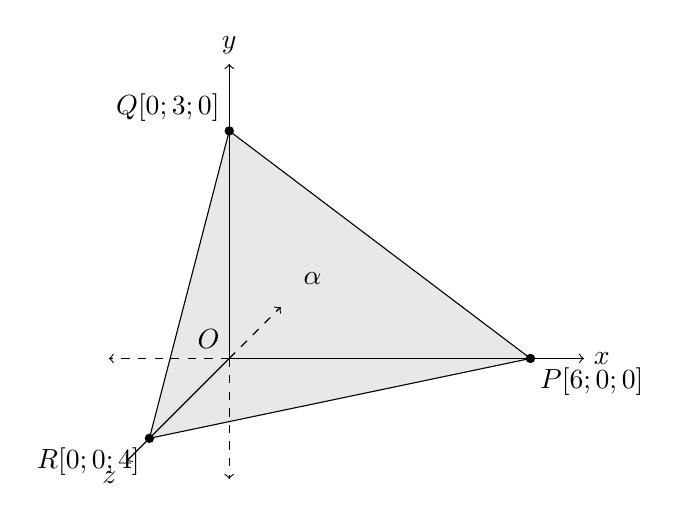
\begin{tikzpicture}[scale=0.85]

        % Průsečíky s osami
        \coordinate (P) at (4.5,0,0);
        \coordinate (Q) at (0,3.4,0);
        \coordinate (R) at (0,0,3.1);

        % Část roviny určená průsečíky
        \fill[gray!18] (P) -- (Q) -- (R) -- cycle;
        \draw[thin] (P) -- (Q) -- (R) -- cycle;

        % Osy - kladná část
        \draw[->] (0,0,0) -- (5.3,0,0) node[right] {$x$};
        \draw[->] (0,0,0) -- (0,4.4,0) node[above] {$y$};
        \draw[->] (0,0,0) -- (0,0,4.0) node[below left] {$z$};

        % Osy - záporná část
        \draw[->, dashed] (0,0,0) -- (-1.8,0,0);
        \draw[->, dashed] (0,0,0) -- (0,-1.8,0);
        \draw[->, dashed] (0,0,0) -- (0,0,-2.0);

        \node[above left] at (0,0,0) {$O$};

        % Body
        \fill (P) circle (2pt) node[below right] {$P[6;0;0]$};
        \fill (Q) circle (2pt) node[above left] {$Q[0;3;0]$};
        \fill (R) circle (2pt) node[below left] {$R[0;0;4]$};

        \node at (1.9,1.85,1.7) {$\alpha$};

    \end{tikzpicture}
    \caption{Rovina určená svými průsečíky se souřadnicovými osami.}
    \label{fig:Plane_intercept_form}
\end{figure}

Úsekový tvar nelze použít v každé situaci. Jestliže je některý
z koeficientů $a$, $b$, $c$ nulový, je rovina rovnoběžná s příslušnou
osou a nemá s ní jediný průsečík. Jestliže rovina prochází počátkem,
je některý z úseků nulový a ve jmenovateli úsekového tvaru by vznikla
nula.

\subsubsection{Shrnutí}
\label{subsubsec:General_plane_summary}

Obecná rovnice roviny má tvar
\[
    ax+by+cz+d=0,
\]
kde alespoň jeden z koeficientů $a$, $b$, $c$ je nenulový.

Z této rovnice můžeme vyčíst normálový vektor
\[
    \vec{n}=(a;b;c).
\]

Bod $P[x_P;y_P;z_P]$ leží v rovině právě tehdy, když po dosazení jeho
souřadnic platí
\[
    ax_P+by_P+cz_P+d=0.
\]

Obecnou rovnici můžeme sestavit zejména tehdy, když známe:

\begin{itemize}
    \item bod roviny a její normálový vektor;
    \item tři nekolineární body roviny;
    \item parametrické vyjádření roviny;
    \item rovinu, se kterou má být hledaná rovina rovnoběžná, a jeden bod;
    \item přímku, ke které má být hledaná rovina kolmá, a jeden bod.
\end{itemize}

Obecná rovnice je vhodná pro ověřování příslušnosti bodů a pro práci
s normálovým směrem roviny. V následujících částech ji využijeme při
zkoumání vzájemné polohy rovin a při určování vztahů mezi přímkami
a rovinami.
